\usepackage{graphicx}\begin{Document}
                         Ezt a szoftvert 2024-ben kezdtem el fejleszteni, de a lényegi részét idén készítettem, folyamatos fejlesztéssel, hibajavítással, kísérletezéssel.


                         Az eredeti beadott verzióval több gond is volt. A programot nem lehetett egy belépési ponttal futtatni. Helyette össze-vissza vide code-olt, kaotikus, gyakran egymástól teljesen független szkriptek szerepeltek mindenhol, amelyeknek a használatát csak én ismertem, ráadásul egy részük nem is működött, csak úgy "volt". A program egyébként is csak a most "ModelInputPreparer"-nek hívott részt tudta lefuttatni standard Python (pl. PyCharm) környezetben. A Hugging Face modell inferenciája (mostani "HuggingFaceModelInferencer") Jupyter Notebookban futott, Google Colab környezetben, majd a modell outputjának feldolgozása (mostani "ModelOutputProcessor") megint egy harmadik környezetben, Google Apps Scriptben került feldolgozásra.
                         Az újraírásnál első lépésem volt, hogy ezt egyesítem. Most az egész szoftver standard Python futtatokornyezetben fut, a könnyen megtalálható "main.py" fájlok futtatásával, ipari standard szerint az src mappában lévő globális belépési ponttal, de egyenként is futtatható a 3 modul.
                         A legnagyobb változást a Clean Code című könyv elolvasása hozta, amely hatására átértékeltem a programozói tudásomat, különös tekintettel a szakdolgozatomra. Láttam, hogy objektum orientált módszerrel nagy szoftvereket is átláthatóan és biztonságosan lehet fejleszteni. Megjegyeztem azt is, hogy a jó elnevezések milyen fontosak. Ezek az elvek alapján írtam meg a vázlatból az új szakdolgozat szoftveremet.
                         A "keretrendszer", bár én inkább modulnak hívom, 3 fő futtatható állományból áll:
                         A ModelInputPreparer, amely a WiC adathalmazból létrehozza a modellnek szánt inputot, az 5600 kérdést. Ez a 'WiC adathalmaz' 'test' splitjének összes rekordjából létrehoz egy kérdést, mind egyenes, mind fordított sorrendben, hogy a modellek konzisztenciáját vizsgáljuk. Mivel 2800 rekordból áll, és rekordonként 2 kérdésünk (egyenes, fordított) van, így jön ki az 5600 kérdés.

% TODO
                         A CloudRunnerNotebooks ...


                         A ModelOutputProcessor ...


                         # Használat:
                         \begin{itemize}
                             \item
                         \end{itemize}
                         példa válasz a `Qwen/Qwen2.5-0.5B-Instruct` futtatására:
                         \begin{figure}
                             \centering
                             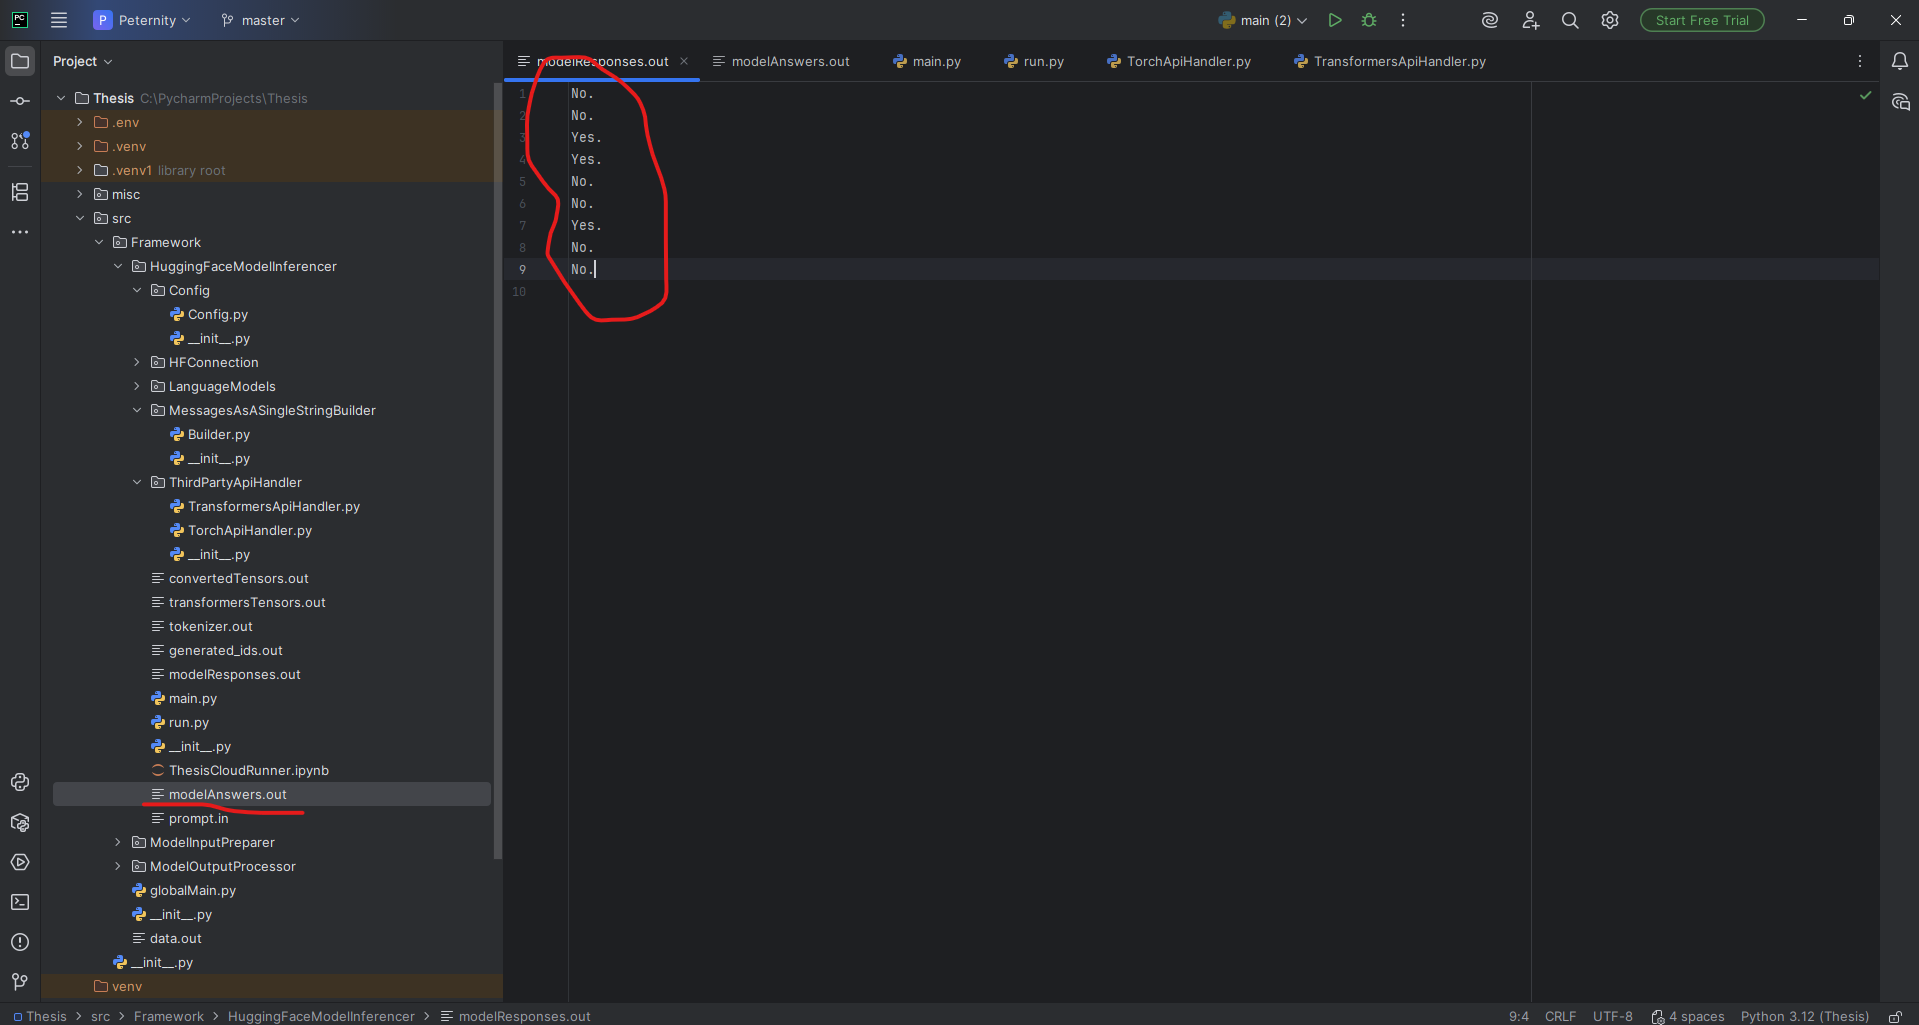
\includegraphics[keepaspectratio]{pelda}
                             \caption{Példa Válasz}
                             \label{fig:PeldaValasz}
                         \end{figure}


\end{Document}